\documentclass[12pt]{article}
\usepackage[top=1in, bottom=1in, left=1in, right=1in]{geometry}

\usepackage{setspace}
\onehalfspacing

\usepackage{amssymb}
%% The amsthm package provides extended theorem environments
\usepackage{amsthm}
\usepackage{epsfig}
\usepackage{times}
\renewcommand{\ttdefault}{cmtt}
\usepackage{amsmath}
\usepackage{graphicx} % for graphics files

% Draw figures yourself
\usepackage{tikz} 

% writing elements
\usepackage{mhchem}

% The float package HAS to load before hyperref
\usepackage{float} % for psuedocode formatting
\usepackage{xspace}

% from Denovo Methods Manual
\usepackage{mathrsfs}
\usepackage[mathcal]{euscript}
\usepackage{color}
\usepackage{array}

\usepackage[pdftex]{hyperref}
\usepackage[parfill]{parskip}

% math syntax
\newcommand{\nth}{n\ensuremath{^{\text{th}}} }
\newcommand{\ve}[1]{\ensuremath{\mathbf{#1}}}
\newcommand{\Macro}{\ensuremath{\Sigma}}
\newcommand{\rvec}{\ensuremath{\vec{r}}}
\newcommand{\vecr}{\ensuremath{\vec{r}}}
\newcommand{\omvec}{\ensuremath{\hat{\Omega}}}
\newcommand{\vOmega}{\ensuremath{\hat{\Omega}}}
\newcommand{\sigs}{\ensuremath{\Sigma_s(\rvec,E'\rightarrow E,\omvec'\rightarrow\omvec)}}
\newcommand{\el}{\ensuremath{\ell}}
\newcommand{\sigso}{\ensuremath{\Sigma_{s,0}}}
\newcommand{\sigsi}{\ensuremath{\Sigma_{s,1}}}
%---------------------------------------------------------------------------
%---------------------------------------------------------------------------
\begin{document}
\begin{center}
{\bf NE 250, F17\\
October 10, 2017 
}
\end{center}

Mid-semester Public Service Announcement: 
\begin{itemize}
\item Grad student mental health resources: \url{http://www.uhs.berkeley.edu/students/counseling/cps.shtml}
\item Sexual assault support on campus: \url{http://survivorsupport.berkeley.edu/}
\end{itemize}

We reached a spot with fission where we can start understanding the balance in the system. What we'll do next is look at criticality from the perspective of how do we perfectly balance materials and geometry -- which will lead us to eigenvalue iterations. 

Before entering into iteration concepts, I wanted to cover some tools beyond diffusion that are used in reactor design. We will end up at both the Method of Characteristics and understanding uncollided and multiply-collided fluxes. Each of these are a valuable complement to the diffusion equation. 

To get there, we will start with \underline{streaming in curvilinear coordinates} for the transport equation. Bear with me through the math. I think it's worth going through because it comes up in what we want to use in the real world, and books often treat other coordinate systems as ``exercises left to the reader." I'd like to actually go through it with you.

This material will come largely from Bell and Glasstone's \textit{Nuclear Reactor Theory} (freely available online) and Lewis and Miller's \textit{Computational Methods of Neutron Transport} (I have a bunch of copies you can borrow). 

With that in mind, here's a reminder of what the TE looks like, where $\psi(\vec{r}, E, \vOmega, t)$ is the angular neutron flux. 
%
\begin{align*}
\frac{1}{v} \frac{d \psi}{dt} &+ \vOmega \cdot \nabla \psi(\vec{r}, E, \vOmega, t) + \Sigma_t \psi(\vec{r}, E, \vOmega, t) = \int_{4 \pi} d\vOmega' \int_0^{\infty} dE' \: \Sigma_s(E', \vOmega' \rightarrow E, \vOmega) \psi(\vec{r}, E', \vOmega', t)\\
 +& \frac{\chi(E)}{4 \pi}\int_0^{\infty} dE' \: \nu(E') \Sigma_f(E') \int_{4 \pi} d\vOmega' \:\psi(\vec{r}, E', \vOmega', t) + S(\vec{r}, E, \vOmega, t)
\end{align*}

How do we manage this equation in \underline{Curvilinear Systems?}
 This is taken from B \& G Chp.\ 1.3.
Recall that $\vOmega \cdot \nabla$ is the derivative of angular flux along the direction of motion $\vOmega$. (See Figure~\ref{fig:cart-coord}).
%
\begin{figure}[h!]
    \begin{center}
    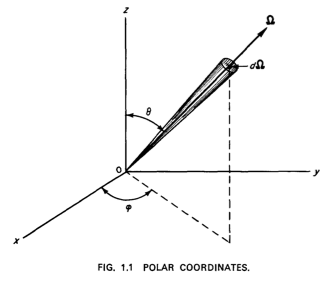
\includegraphics[keepaspectratio, width = 3.75 in]{../figs/polar-coords}
    \end{center}   
    \caption{Polar Coordiantes}
    \label{fig:cart-coord}
\end{figure}
%
\begin{align*}
\vOmega &= \Omega_x + \Omega_y + \Omega_z =  \sin(\theta)\cos(\varphi) + \sin(\theta)\sin(\varphi) + \cos(\theta)\\
\nabla &= \hat{e}_1 \underbrace{\mathcal{D}_1}_{\text{derivative in direction }\hat{e}_1} + \hat{e}_2 \mathcal{D}_2 + \hat{e}_3 \mathcal{D}_3\\
&= \hat{e}_1 \frac{d}{dx} + \hat{e}_2 \frac{d}{dy} + \hat{e}_3 \frac{d}{dz} \quad \text{in Cartesian}
\end{align*}

\begin{figure}[h!]
    \begin{center}
    \includegraphics[keepaspectratio, width = 4.25 in]{../figs/n-motion-sph}
    \end{center}    
    \caption{Streaming in Spherical Coordinates}
    \label{fig:sph-m} 
\end{figure}

In curvilinear geometry, neutrons ``migrate" across $\vOmega$ as they stream in straight lines. 
We can see this in spherical geometry (note: $dr$, $d\theta$, and $ds$ are assumed to be very small). We will use Figure~\ref{fig:sph-m} to understand our derivatives. Also recall sin = O/H, cos = A/H, and $\sin^2 + \cos^2 = 1$. Also recall that $\vOmega \cdot \hat{\vec{r}} = \mu$.
%
\begin{align*}
\frac{d \psi}{ds} &= \frac{d \psi}{dr} \frac{dr}{ds} + \frac{d\psi}{d\mu} \frac{d\mu}{ds} \\
&\text{Look at the figure to define the terms}\\
\frac{dr}{ds} &= \cos(\theta) = \mu \\
%
\frac{d \mu}{ds} &= -\sin(\theta) \frac{d \theta}{ds} = -\sin(\theta) \biggl(\frac{-\sin(\theta)}{r} \biggr) = \biggl(\frac{1 - \mu^2}{r} \biggr) \\
%
\frac{d\psi}{ds} &= \mu \frac{\partial \psi}{\partial r} + \underbrace{\frac{(1 - \mu^2)}{r}\frac{\partial \psi}{\partial \mu}}_{\text{redistribution term}}
\end{align*}

We can combine all of that we get the ``conservation form" of the derivative term (see B\&G 1.3b for derivation)
\[\frac{d\psi}{ds} = \frac{\mu}{r^2} \frac{\partial(r^2 \psi)}{\partial r} + \frac{1}{r} \frac{\partial}{\partial \mu}\bigl[(1 - \mu^2) \psi \bigr] \:. \]

I've included a table of the spherical conservative form terms as well as the coordinate system and conservative form for cylindrical coordinates in the notes.
%
\begin{figure}[h!] 
    \label{fig:sph-op}
    \begin{center}
    \includegraphics[keepaspectratio, width = 7 in]{../figs/spherical-operator}
    \end{center}    
    \begin{center}
    \includegraphics[keepaspectratio, width = 4 in]{../figs/cyl-coords}
    \end{center}    
    \label{fig:cyl-coord}
    \begin{center}
    \includegraphics[keepaspectratio, width = 5 in]{../figs/cyl-operator}
    \end{center}    
    \caption{Spherical and Cylindrical terms: L\&M Chp.\ 1}
\end{figure}




\end{document}
